\chapter{Theory}
\label{chapter:theory}


\noindent\lipsum[20-25]

\section{Example Figure}
Make sure to include pdf format (or any vector graphics format) figures in your thesis whenever possible. You will be thankful for it when printing the document. 
\begin{figure}[H]
    %% trim=left bottom right top,
    \centering
   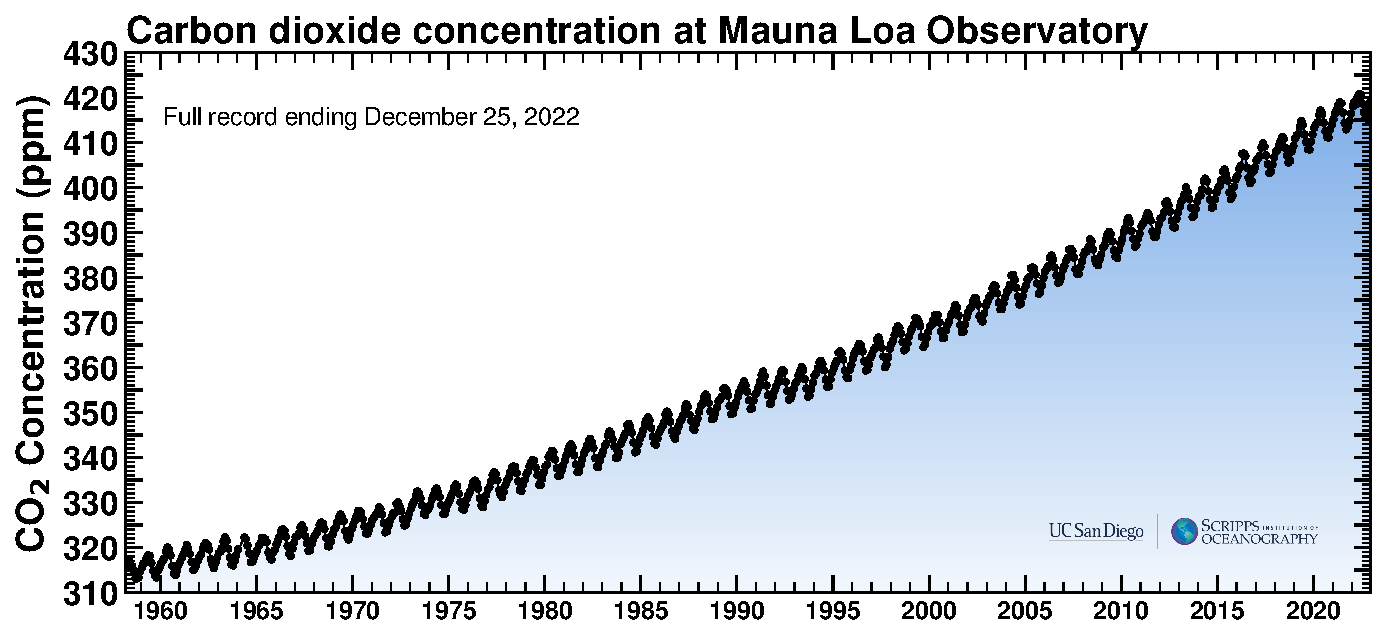
\includegraphics[width=1.0\textwidth,keepaspectratio,trim=0 0 0 0, clip]{figures/mlo_full_record.pdf}
    \caption{ Mauna Loa observatory \ch{CO2} measurement \parencite{keeling-curve} }
    \label{fig:scatter_plot_sand}
\end{figure}


\section{Example chemical reaction}
Carbonic acid deprotonation:
\begin{equation}
    \ch{CO2 + H2O ->[] HCO3^- + H^+}.
\end{equation}

\section{Example of the equation with self-defined conditions environment }
The relative permittivity $\epsilon_{r}$ is defined as: 
\begin{equation}
    \label{eqn:relative_permittivity}
    {\displaystyle \varepsilon _{\mathrm {r} }={\frac {\varepsilon }{\varepsilon _{0}}}}
\end{equation}
\begin{conditions}
    \epsilon & permittivity of the material \\
    \epsilon_0 & vacuum permittivity.\\
\end{conditions}

\section{Example of different citations}
Overall \textcite{arrhenius1896xxxi} calculated that cutting CO2 in half would suffice to produce an ice age. He further calculated that a doubling of atmospheric CO2 would give a total warming of 5–6 degrees Celsius.

\noindent
Overall, Arrhenius calculated that cutting CO2 in half would suffice to produce an ice age. He further calculated that a doubling of atmospheric CO2 would give a total warming of 5–6 degrees Celsius (\cite{arrhenius1896xxxi}).

\noindent
Overall, Arrhenius calculated that cutting CO2 in half would suffice to produce an ice age. He further calculated that a doubling of atmospheric CO2 would give a total warming of 5–6 degrees Celsius \parencite{arrhenius1896xxxi}.

\section{Example list}
\begin{itemize}
    \item first
    \item second
    \item third
    \item fourth
    \item fifth
    \item sixth
    \item seventh
\end{itemize}

\section{Example table}

\begin{table}[H]
\centering
\begin{tabular}{|l|l|}
\hline
\rowcolor{gray!50}
Country (or dependency) & Population (2020) \\ \hline
China                  & 1,439,323,776       \\ \hline
India                  & 1,380,004,385        \\ \hline
USA                    & 331,002,651           \\ \hline
Indonesia              & 273,523,615            \\ \hline
Pakistan               & 220,892,340             \\ \hline
Brazil                 & 212,559,417              \\ \hline
Nigeria                & 206,139,589               \\ \hline
\end{tabular}
\caption{example caption }
\label{tbl:example_table}
\end{table}

\section{Example of siunitx package}
The siunitx package is amazing for controlling all numbers and units of the document globally. You can set everything globally for the document and don't need to change every single number for formatting changes.\\
At the beginning of the document, the settings are made.

%% settings for the SI units from main.tex
% \sisetup{locale = DE,
% output-decimal-marker={.}, % because  in german is switched to {,}
% separate-uncertainty=true,  
% multi-part-units=single,
% range-units = single ,  
% list-units = single,  
% per-mode=reciprocal,
% group-minimum-digits = 4,
% number-unit-product = \hspace{0.16667em plus 0.08334em}}



\begin{itemize}
    \item range of numbers + unit:  \SIrange{3}{10}{\cubic\kilo\meter \per \second}
    \item number + unit : \SI{3}{\cubic\kilo\meter \per \second}
    \item just unit   : \si{\cubic\kilo\meter \per \second}
    \item number + uncertainty + unit \SI{3 \pm 0.1}{\cubic\kilo\meter \per \second}
\end{itemize}

\section{Example colors}
Example of how to use colors in the text.
\begin{enumerate}
\color{blue}
    \item Blue
    \item More blue
    \item {\color{red} And red!}
    \item \begingroup\color{green} lol   \endgroup
    \item {\color{yellow} And yellow!}
\end{enumerate}


